\documentclass{standalone}

\usepackage{tikz}

\begin{document}

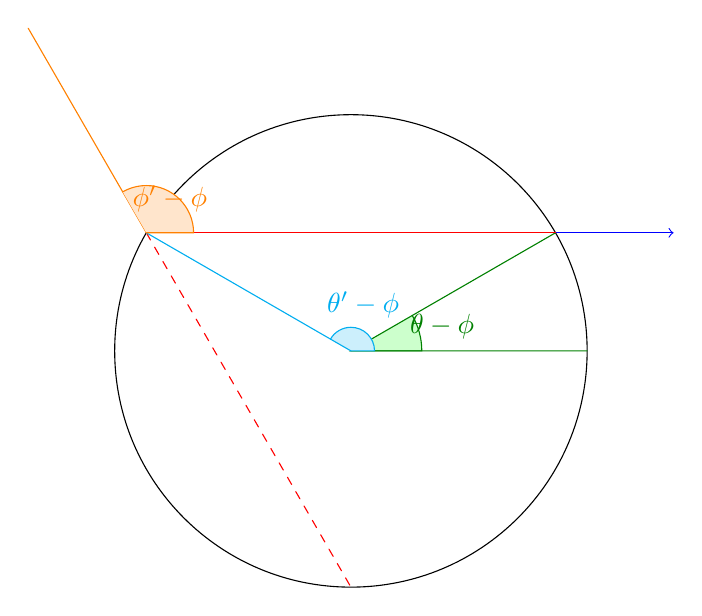
\begin{tikzpicture}[scale=3,cap=round]

    \colorlet{thetacolor}{green!50!black}
    \colorlet{phicolor}{blue}
    \colorlet{lcolor}{red}

    \draw (0,0) circle (1cm);

    \filldraw[fill=green!20,draw=thetacolor] (0,0) -- (3mm,0pt) arc(0:30:3mm);
    \draw (15:4mm) node[thetacolor] {$\theta-\phi$};

    \draw[thetacolor] (30:1cm) -- (0,0) -- (1cm, 0);

    \draw[->,phicolor] (30:1cm) -- +(0.5,0);

    \draw[lcolor] (30:1cm) -- (150:1cm);
    \draw[lcolor, dashed] (150:1) -- (-90:1);

    \filldraw[fill=cyan!20,draw=cyan] (0,0) -- (1mm,0pt) arc(0:150:1mm);
    \draw (75:2mm) node[cyan] {$\theta'-\phi$};

    \draw[cyan] (0,0) -- (150:1);

    \draw[orange] (150:1) -- +(-0.5, 0.866);
    \filldraw[fill=orange!20,draw=orange] (-0.866,0.5) -- (-0.666,0.5) arc(0:120:2mm);
    \draw (140:1) node[orange] {$\phi'-\phi$};


\end{tikzpicture}

\end{document}